\chapterimage{anexos/1_lenguajes_marcado/1_markdown/imagenes/cover.jpg}
\chapterimagedescription{Logo de Markdown sobre fondo con logos tridimensionales}
\chapterimageauthor{Diseño propio}

\chapter{Markdown}
\index{Markdown}
\label{anex:markdown}

\textbf{Markdown} es un lenguaje de marcado ligero creado por \textbf{John Gruber},
con ayuda de \textbf{Aaron Swartz}, que trata de conseguir la máxima legibilidad
y facilidad de publicación tanto en su forma de entrada como de salida. Gruber
deseaba que la gente pudiera escribir un documento de forma sencilla, y que
pudiera comprenderlos, sin necesidad de saber demasiado sobre el lenguaje, y
aún así producir documentos válidos que pudieran ser exportados luego a documentos
HTML válidos.

Si bien su lanzamiento oficial fue en el 2004, se inspira en una gran cantidad
de convenciones existentes para marcar mensajes de correo electrónico en texto
plano, muy utilizadas en la década de 1980 y principios de 1990. Markdown es un
lenguaje libre, y también lo son sus herramientas, que se distribuyen bajo una
\textbf{licencia BSD}. La versión original fue creada en el lenguaje de
programación Perl, pero con el tiempo se ha portado a muchos otros lenguajes.

No hay un estándar definido para Markdown, aparte de la implementación original
de John Gruber, que algunos consideran obsoleto. Esto ha ocasionado una gran
fragmentación, con diversas implementaciones que agregan funciones, o remueven
otras.

Markdown se ha posicionado como un importante lenguaje en diversos ámbitos, por
ejemplo, varios sistemas de blogs permiten escribir artículos utilizando
Markdown.

En el área de programación es ampliamente utilizado para escribir documentación
de los programas, convirtiéndose en el estándar de facto. Por ejemplo,
sitios que albergan repositorios de código, como \textbf{GitHub}, \textbf{GitLab}
y \textbf{Bitbucket} entre otros, incluyen visualizadores para Markdown que
muestran la documentación del programa de forma automática. Cómo estos sitios
albergan proyectos de software libre, leer la documentación de estos programas
es una buena forma de aprender Markdown, ya que se puede ver fácilmente la
visualización y su código fuente.

También cabe destacar que, si bien se puede escribir código Markdown con cualquier
editor de texto simple, existen editores especializados o plugins para editores
que permiten visualizar la salida como HTML, resaltan la sintaxis y proveen
funciones de autocompletado. También existen editores con visualizadores que
corren directamente online, sin necesidad de instalar nada en el equipo,
como el sitio web \href{http://dillinger.io/}{http://dillinger.io/}.

Los archivos que contienen código markdown suelen guardarse con la extensión
\textbf{.md}, o con extensión \textbf{.markdown}, según la herramienta que se
utilice para producirlos.

Cabe destacar que Markdown permite exportar el contenido a HTML, un lenguaje
de marcado que se utiliza para diseñar páginas web. Sin embargo, sus características
están muy reducidas con respecto a este último, por lo que el diseño de páginas
no es su función. En cambio, está pensado para redactar correos electrónicos,
artículos simples y documentación.

\section{Sintaxis y Semántica}

\subsection*{Párrafos y texto simple}

Todo texto escrito en un documento Markdown que no contenga marcas específicas
aparece tal cual, como un párrafo. Un salto de línea en el texto original
no se ve reflejado en el resultado visualizado.

Los saltos de línea en la salida se dan cuando se insertan dos espacios
consecutivos en la entrada (donde un salto de línea es considerado un espacio).

\begin{lstlisting}[language=Markdown]
Esto es un párrafo único, incluso
si hay un salto de línea en el medio.

Esto aparece en otro párrafo, pues hay dos
saltos de línea desde el párrafo anterior.
\end{lstlisting}

\subsection*{Énfasis}

Existen dos formas de enfatizar una palabra en Markdown, un énfasis simple
(que en general se visualiza como texto en itálica), y un énfasis doble (
para palabras o frases un poco más importantes que las anteriores, y que se
termina visualizando en negrita).

El énfasis consiste en colocar una marca (para énfasis simple) o dos (para énfasis
doble) al inicio del texto a resaltar, y la misma cantidad al final de dicho texto.
Pueden utilizarse tanto guiones bajos como asteriscos para marcar, pero en general
se estila utilizar guión bajo para énfasis simple, y asteriscos para negrita.

\begin{lstlisting}[language=Markdown]
Esto texto _tiene estas palabras con énfasis simple_,
pero estas que están a continuación **Presentan énfasis doble**
\end{lstlisting}

La salida del texto anterior se visualizará de forma similar
a lo siguiente:

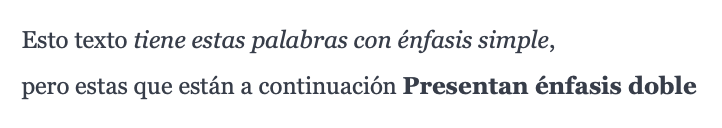
\includegraphics[]{anexos/1_lenguajes_marcado/1_markdown/imagenes/md_enfasis.png}

\subsection*{Títulos}

Los títulos permiten delimitar secciones bien diferenciadas en el texto,
y ya son por si mismos texto resaltado, por lo que no deben rodearse de
marcas de énfasis.

Los títulos vienen en diversos niveles, de acuerdo a la importancia del
mismo. Por ejemplo, los títulos de primer nivel son los más importantes,
y por tanto deberían ser utilizados solo como el título general del documento.
Los títulos de nivel dos actúan como subtitulo, y permiten diferenciar
secciones grandes del documento. Títulos de tercer, cuarto, quinto y sexto
nivel pueden ser utilizados para marcar secciones más especificas.

Los títulos, si bien tienen un estilo destacado, tienen una connotación
semántica clara. No deberían ser utilizados para enfatizar palabras.

Los títulos comienzan con uno o más signos de numeral, llamado también
almohadilla, o hash (\#). La cantidad de almohadillas expresa el nivel
del título, siendo una almohadilla los títulos de primer nivel, dos almohadillas
de segundo nivel, y así siguiendo.

\begin{lstlisting}[language=Markdown]
# Título de primer nivel
## Título de segundo nivel
### Título de tercer nivel
#### Título de cuarto nivel
##### Título de quinto nivel
###### Título de sexto nivel
\end{lstlisting}

Lo que se termina visualizando como:

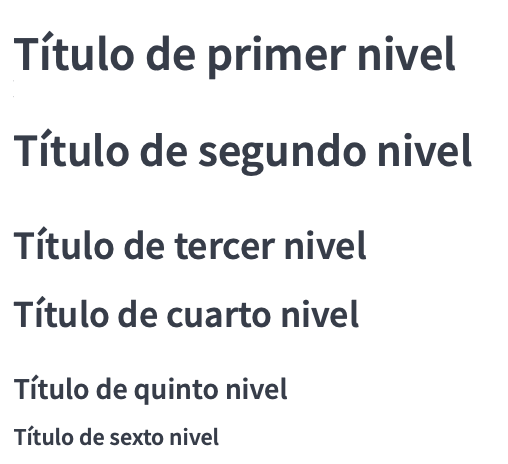
\includegraphics[]{anexos/1_lenguajes_marcado/1_markdown/imagenes/md_titulos.png}

También existe una forma distinta de escribir títulos de primer y segundo
nivel, que consiste en ``subrayar'' las palabras que conforman el texto.
Un subrayado doble indica títulos de primer nivel, y se logra utilizando
signos de igual (=) para realizar el subrayado. Un subrayado simple indica
títulos de segundo nivel, y se logra utilizando guiones medios, o signos de
resta (-). El subrayado debe tener al menos dos signos consecutivos, pero
lo ideal para maximizar la lectura en la entrada es que abarque tanto como
el texto que está marcando.

\begin{lstlisting}[language=Markdown,otherkeywords={=,-},morekeywords={[2]{=,-}}]
Título de primer nivel
======================

Título de segundo nivel
-----------------------
\end{lstlisting}

\subsection*{Listas no ordenadas}

Las listas no ordenadas marcan cada uno de sus elementos como viñetas.
Se pueden utilizar asteriscos (*), signos de suma (+), o guiones o signos
de resta (-) para marcar los elementos de la lista. Incluso pueden combinarse,
aunque esto atenta contra la lectura en la entrada y no es recomendado.

\begin{lstlisting}[language=Markdown,otherkeywords={+},morekeywords={[2]{+}}]
+ Item 1
+ Item 2
+ Item 3
\end{lstlisting}

Resulta en:

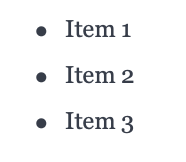
\includegraphics[]{anexos/1_lenguajes_marcado/1_markdown/imagenes/md_ulist_1.png}

También pueden colocarse listas dentro de otras listas, tabulando los
elementos

\begin{lstlisting}[language=Markdown,otherkeywords={+},morekeywords={[2]{+}}]
+ Item 1
+ Item 2 tiene los siguientes elementos
    * Item 2A
    * Item 2B
+ Item 3
\end{lstlisting}

Resultando en:

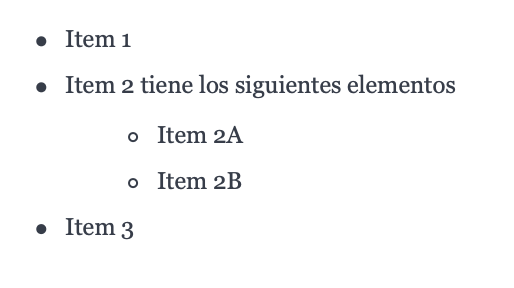
\includegraphics[]{anexos/1_lenguajes_marcado/1_markdown/imagenes/md_ulist_2.png}

\subsection*{Listas ordenadas}

Las listas ordenadas, también llamadas listas numeradas, presentan números
en lugar de viñetas. Se logran colocando un número al comienzo de la línea
y siguiéndolo de un punto.

\begin{lstlisting}[language=Markdown]
1. Primer elemento
2. Segundo elemento
3. Tercer elemento
\end{lstlisting}

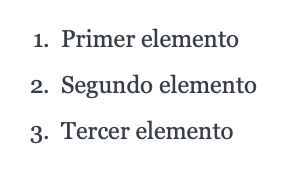
\includegraphics[]{anexos/1_lenguajes_marcado/1_markdown/imagenes/md_olist.png}

De igual forma que con las listas desordenadas, estas se pueden anidar. Más
aún, se pueden anidar listas ordenadas con no ordenadas en diversas formas.

\subsection*{Enlaces}

Una característica interesante es la posibilidad de insertar enlaces en cualquier
punto del texto, que apuntan a otros documentos o sitios web. Un enlace se compone
de dos partes: la dirección a la cual se quiere acceder, y el texto que se le
mostrará al lector. El texto se coloca entre corchetes, los cuales van seguidos
de unos paréntesis que contienen la dirección a la cual se enlazará.

\begin{lstlisting}[language=Markdown]
Lo siguiente es un enlace: [Ir a Google](https://google.com)
\end{lstlisting}


\includegraphics[]{anexos/1_lenguajes_marcado/1_markdown/imagenes/md_enlace.png}

\subsection*{Imágenes}

En ocasiones es necesario agregar algún tipo de elemento visual, en particular,
imágenes. Las imágenes funcionan de forma similar a un enlace, pero se debe
anteponer un signo de admiración (!) a los corchetes. El texto que se coloca
entre corchetes corresponde con la descripción de la imagen, mientras que la
dirección entre paréntesis corresponde con la ubicación de la misma.

\begin{lstlisting}[language=Markdown]
![Logo de Markdown Here](http://cor.to/mdhere)
\end{lstlisting}


\includegraphics[scale=0.4]{anexos/1_lenguajes_marcado/1_markdown/imagenes/md_imagen.png}

\subsection*{Código}

Por haber sido pensado para escribir documentación de código de programación,
Markdown incluye una forma de mostrar código. Para ello se utilizan comillas
agudas, llamadas también backsticks (`). El texto entre backsticks se corresponde
a código fuente. Si el mismo tiene varias líneas, se deben incluir tres backsticks
en lugar de uno, pudiendo colocar al final de los backsticks de apertura,
en el inicio y entre corchetes, el lenguaje en el que se está escribiendo el código.

\begin{lstlisting}[language=Markdown]
`let x = 5`

``` [JavaScript]
let x = 5;
let y = 7;
let z = x + y;
```
\end{lstlisting}

Lo cual se vería así:

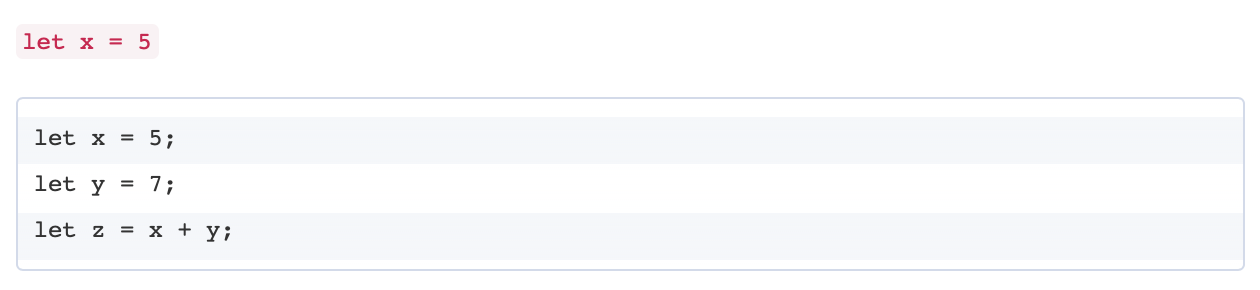
\includegraphics[scale=0.63]{anexos/1_lenguajes_marcado/1_markdown/imagenes/md_codigo.png}

\subsection*{Separaciones}

También es posible colocar líneas de separación entre diferentes secciones del
texto. Una línea de separación se ve como una fina línea horizontal que abarca
todo el ancho del documento, y puede hacerse con una serie de signos de resta o
guiones (-) colocados de forma consecutiva.

También pueden utilizarse asteriscos o signos de igual para la separación.

\begin{lstlisting}[language=Markdown]
Esta sección se encuentra separada de la que le sigue.

------------------------------------------------------

La línea superior marca esa separación de forma clara.
\end{lstlisting}


\section{Actividades}

\begin{exercise}
Dado el siguiente código en Markdown, modifique el mismo de forma tal de dar
énfasis simple a los periféricos que aparecen mencionados y énfasis doble a las
palabras informática, software y hardware en todos los lugares en donde aparece.

\begin{minipage}{0.92\textwidth}
    \begin{lstlisting}[language=Markdown]
La informática es la disciplina que que estudia el
tratamiento automatizado de información por parte
de las computadoras, las cuales se componen de un
conjunto de hardware y software.

El hardware se compone de una placa base, una
fuente de alimentación, memoria, un microprocesador,
y un conjunto de periféricos tales como mouse,
teclado, pantalla, parlantes, impresora, micrófono
y placas de expansión.

El software consiste en los programas que corremos
en el equipo, como Word, GIMP, Age of Empires y otros.
    \end{lstlisting}
\end{minipage}
\end{exercise}

\begin{exercise}
Redacte en Markdown una receta para hacer tallarines caseros, utilizando una
lista no ordenada para los mencionar los ingredientes y una lista ordenada para
los pasos a seguir en la preparación. Puede valerse de Internet para buscar una
receta, en caso de que desconozca los pasos a seguir.
\end{exercise}

\begin{exercise}
Busque en Internet imágenes de tres lugares del mundo que desearía visitar.
En un documento Markdown, inserte las imágenes de forma consecutiva, colocando
previo a cada una el nombre del lugar como titulo de nivel 3, y el país en el
que se encuentra como subtitulo de nivel 5. El título debe consistir en un enlace
a la página de Wikipedia sobre ese lugar.
\end{exercise}

\begin{exercise}
El siguiente código Markdown tiene algunos errores, tanto semánticos como de
sintaxis.

\begin{minipage}{0.92\textwidth}
\begin{lstlisting}[language=Markdown]
##### Sobre Markdown

## El lenguaje

El lenguaje Markdown fue creado en 2004 por John Gruber.
Es un lenguaje de marcado ligero diseñado para maximizar la
facilidad de escritura y lectura tanto en la entrada como
en la salida.

-----------------------------------------------

## _La sintaxis_

La sintaxis del lenguaje es sencilla, y consiste en signos
como asteriscos, almohadillas, y corchetes para lograr
estructurar un documento. En general se pueden escribir
los elementos de la siguiente lista:

Títulos
Palabras con énfasis
Listas
Enlaces
Código

-----------------------------------------------

Copyright 2019
\end{lstlisting}
\end{minipage}

Se pide entonces que detecte los errores y proponga un código que los corrija.
\end{exercise}

\begin{exercise}
Elabore un documento Markdown que funcione como su curriculum vitae.
Para ello, coloque su nombre completo como título principal, y siga al mismo
con un subtitulo de nivel dos indicando su profesión. Agregue una foto de su persona,
y seccione el contenido en datos personales, trabajos, formación y otros elementos
utilizando títulos de tercer nivel en adelante y separadores según lo considere
necesario. Utilice una lista no ordenada para sus datos personales.

No hace falta que el CV sea real, basta con que sea verosímil, si no cuenta con
experiencia laboral o estudios, puede inventarlos para realizar esta actividad.
\end{exercise}

\begin{exercise}
Realice en Markdown una breve carta de presentación donde usted solicita
un puesto de ``Desarrollador de Software'' en una empresa. Utilice títulos,
énfasis y listas de forma apropiada en los lugares que crea conveniente.
\end{exercise}
